\documentclass[letterpaper,12pt]{article}

% \usepackage[margin=1in]{geometry}
\usepackage{geometry}
% \usepackage{lipsum}
%
% \usepackage{hyperref}
%
\usepackage{graphicx}
\graphicspath{ {images/} }
\synctex=1


% \bibliographystyle{IEEEtran}

\usepackage[utf8x]{inputenc}
\usepackage{float}

\title{ECE 321: Software Requirements Engineering \\ Assignment 3}
\author{Arun Woosaree \\ \\ XXXXXXX}

\begin{document}
\maketitle
% \newpage

\section{}
\begin{figure}[H]
 \centering
 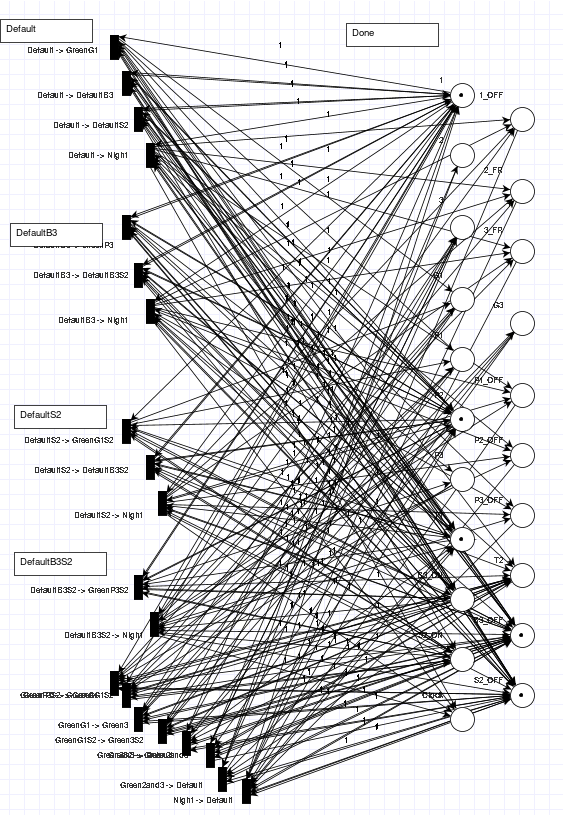
\includegraphics[width=\textwidth]{petrinet.png}
 \caption{Screenshot of the petri net created in PIPE}
 % \label{q6}
\end{figure}

\begin{figure}[H]
 \centering
 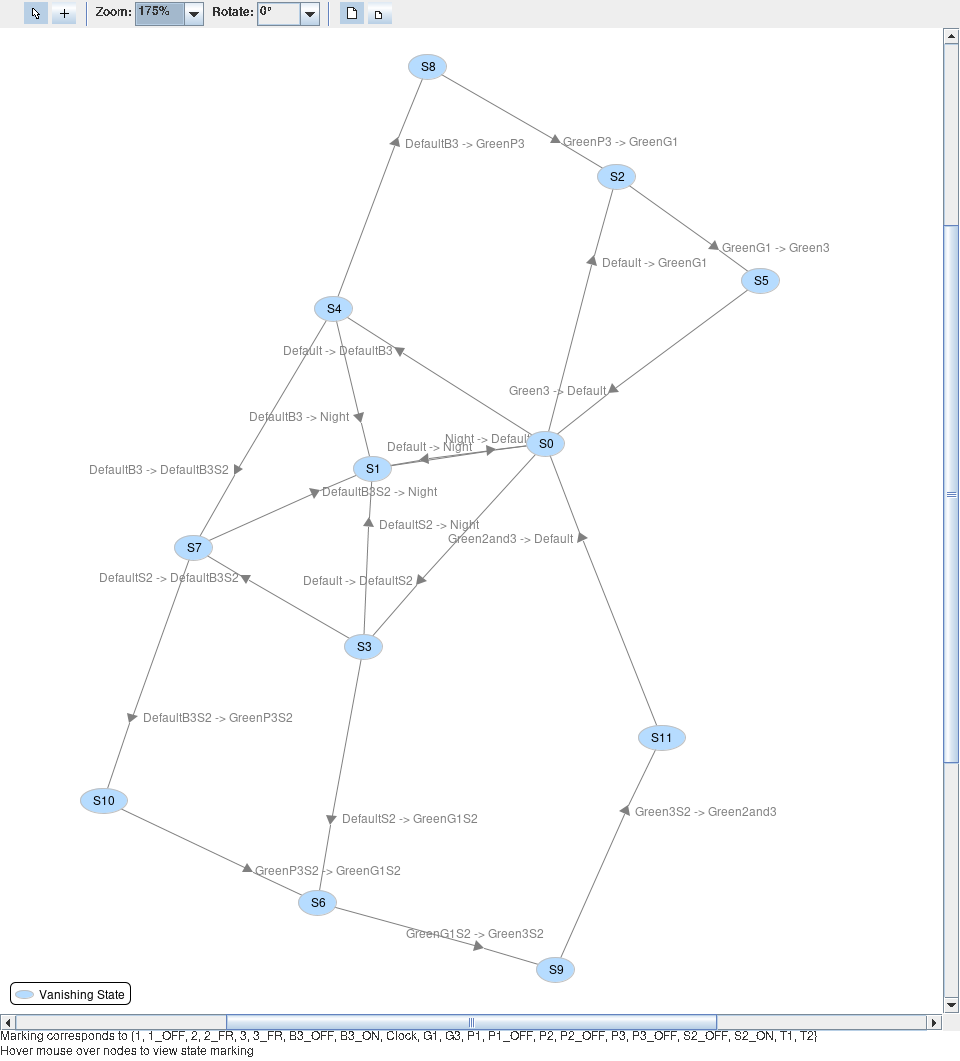
\includegraphics[width=\textwidth]{reachabilitygraph.png}
 \caption{Screenshot of the reachability graph generated from the petri net}
 % \label{q6}
\end{figure}


\section{Description of transitions}

% Please add the following required packages to your document preamble:
% \usepackage{graphicx}
\begin{table}[]
 \centering
 \resizebox{\textwidth}{!}{%
  \begin{tabular}{|c|c|c|c|c|c|c|c|c|c|c|c|c|c|c|c|c|c|c|c|c|c|}
   \hline
               & 1 & 1\_OFF & 2 & 2\_FR & 3 & 3\_FR & G1 & G3 & P1\_ON & P1\_OFF & P2\_ON & P2\_OFF & P3\_ON & P3\_OFF & T1 & T2 & B3\_ON & B3\_OFF & S2\_ON & S2\_OFF & Clock \\ \hline
   Default     & 1 & 0      & 0 & 0     & 0 & 0     & 0  & 0  & 0      & 0       & 1      & 0       & 0      & 0       & 1  & 0  & 0      & 1       & 0      & 1       & 0     \\ \hline
   DefaultB3   & 1 & 0      & 0 & 0     & 0 & 0     & 0  & 0  & 0      & 0       & 1      & 0       & 0      & 0       & 1  & 0  & 1      & 0       & 0      & 1       & 0     \\ \hline
   DefaultS2   & 1 & 0      & 0 & 0     & 0 & 0     & 0  & 0  & 0      & 0       & 1      & 0       & 0      & 0       & 1  & 0  & 0      & 1       & 1      & 0       & 0     \\ \hline
   DefaultB3S2 & 1 & 0      & 0 & 0     & 0 & 0     & 0  & 0  & 0      & 0       & 1      & 0       & 0      & 0       & 1  & 0  & 1      & 0       & 1      & 0       & 0     \\ \hline
   GreenP3     & 1 & 0      & 0 & 0     & 0 & 0     & 0  & 0  & 0      & 0       & 1      & 0       & 1      & 0       & 0  & 1  & 1      & 0       & 0      & 1       & 0     \\ \hline
   GreenP3S2   & 1 & 0      & 0 & 0     & 0 & 0     & 0  & 0  & 0      & 0       & 1      & 0       & 1      & 0       & 0  & 1  & 1      & 0       & 1      & 0       & 0     \\ \hline
   GreenG1     & 0 & 0      & 0 & 0     & 0 & 0     & 1  & 0  & 1      & 0       & 0      & 0       & 0      & 0       & 0  & 1  & 0      & 1       & 0      & 1       & 0     \\ \hline
   GreenG1S2   & 0 & 0      & 0 & 0     & 0 & 0     & 1  & 0  & 1      & 0       & 0      & 0       & 0      & 0       & 0  & 1  & 0      & 1       & 1      & 0       & 0     \\ \hline
   Green3      & 0 & 0      & 0 & 0     & 1 & 0     & 0  & 1  & 0      & 0       & 0      & 0       & 0      & 0       & 0  & 1  & 0      & 1       & 0      & 1       & 0     \\ \hline
   Green3S2    & 0 & 0      & 0 & 0     & 1 & 0     & 0  & 1  & 0      & 0       & 0      & 0       & 0      & 0       & 0  & 1  & 0      & 1       & 1      & 0       & 0     \\ \hline
   Green2and3  & 0 & 0      & 1 & 0     & 1 & 0     & 0  & 0  & 0      & 0       & 0      & 0       & 0      & 0       & 0  & 1  & 0      & 1       & 0      & 1       & 0     \\ \hline
  \end{tabular}%
 }
 \caption{A table indicating where tokens should be for each state (1 represents 1 token, and 0 represents no tokens)}
 \label{my-label}
\end{table}

\begin{enumerate}
 \item Default $\rightarrow$ GreenG1\\
       This transition happens when the system is in the default state and timer T1 fires.
 \item Default $\rightarrow$ DefaultB3\\
       This transition happens when the system is in the default state and a pedestrian hits the button B3
 \item Default $\rightarrow$ DefaultS2\\
       This transition happens when the system is in the default state and a vehicle is detected on sensor S2
 \item Default $\rightarrow$ Night\\
       This transition happens when the system is in the default state and the clock indicates nighttime
 \item DefaultB3 $\rightarrow$ GreenP3\\
       This transition happens when the system is in the DefaultB3 state and timer T1 fires.
       DefaultB3 is similar to the Default state, except that a pedestrian hit the button B3.
 \item DefaultB3 $\rightarrow$ DefaultB3S2\\
       This transition happens when the system is in the DefaultB3S2 state, and a vehicle is detected on sensor S2. DefaultB3 is similar to the Default state, except that a pedestrian hit the button B3.
 \item DefaultB3 $\rightarrow$ Night\\
       This transition happens when the system is in the DefaultB3 state and the clock indicates nighttime
 \item DefaultS2 $\rightarrow$ GreenG1S2\\
       This transition happens when the system is in the DefaultB3 state and timer T1 fires.
       This is similar to the transition Default $\rightarrow$ GreenG1, except that a vehicle
       is detected on sensor S2
 \item DefaultS2 $\rightarrow$ DefaultB3S2\\
       This transition happens when the system is in the DefaulS2 state, and a vehicle is detected on sensor S2. DefaultB3S2 is similar to the Default state, except that a pedestrian hit the button B3, and a vehicle is detected on sensor S2.
 \item DefaultS2 $\rightarrow$ Night\\
       This transition happens when the system is in the DefaultS2 state and the clock indicates nighttime
 \item DefaultB3S2 $\rightarrow$ GreenP3S2\\
       This transition happens when the system is in the DefaultB3S2 state and timer T1 fires.
       This is similar to the transition Default $\rightarrow$ GreenG1, except that a vehicle
       was detected on sensor 2 and a pedestrian requested to cross
 \item DefaultB3S2 $\rightarrow$ Night\\
       This transition happens when the system is in the DefaultB3S2 state and the clock indicates nighttime
 \item GreenP3 $\rightarrow$ GreenG1\\
       This transition happens when the system is in the GreenP3 state and timer T2 fires
 \item GreenP3S2 $\rightarrow$ GreenG1S2\\
       This transition happens when the system is in the GreenP3 state and timer T2 fires.
       This is very similar to the transition above, except that a vehicle was detected
       on sensor S2
 \item GreenG1 $\rightarrow$ Green3\\
       This transition happens when the system is in the Green3 state and timer T2 fires.
 \item GreenG1S2 $\rightarrow$ Green3S2\\
       This transition happens when the system is in the GreenG1S2 state and timer T2 fires.
       This is very similar to the transition above, except that a vehicle was detected
       on sensor S2
 \item Green3 $\rightarrow$ Default\\
       This transition happens when the system is in the Green3 state and timer T2 fires.
 \item Green3S2 $\rightarrow$ Green2and3\\
       This transition happens when the system is in the Green3 state and timer T2 fires.
       This is similar to the transition above, except that a vehicle was detected
       on sensor S2, so we go to state Green2and3 before returning to the default state
 \item Green2and3 $\rightarrow$ Default\\
       This transition happens when the system is in the Green2and3 state and timer T2 fires.
 \item Night $\rightarrow$ Default\\
       This transition happens when the clock signals daytime, and it was previously night.
\end{enumerate}
\section{}

\subsection{Is the model conservative?}
We can clearly see that the number of tokens in the petri net is not constant,
therefore the model is not conservative.

\subsection{Can we have deadlock?}
Using the \textit{Space analysis tool} in PIPE, we see that the model is bounded, safe, and has no deadlock.

\subsection{Can we have starvation?}
Yes, the model can have starvation
The transitions are as follows:
\begin{enumerate}
 \item Default $\rightarrow$ GreenG1
 \item GreenG1 $\rightarrow$ Green3
 \item Green3 $\rightarrow$ Default\\
       ...
\end{enumerate}
Starvation can be prevented here by adjusting the firing times of the timers.


\end{document}
